\documentclass[conference]{IEEEtran}

\usepackage{graphicx}
\usepackage{xcolor}
\usepackage{amsmath,amssymb}
\usepackage{booktabs}
\usepackage{siunitx}
\usepackage[hidelinks]{hyperref}
\usepackage[section]{placeins} % フロートをセクション内に制限
\usepackage{tikz}
\usetikzlibrary{calc,positioning,arrows.meta,shapes.geometric,fit}

% TikZ 共通スタイル
\tikzset{
  >=Latex,
  block/.style = {draw, rounded corners, minimum height=8mm, inner sep=2.5mm},
  box/.style   = {draw, rounded corners, inner sep=2mm},
  small/.style = {font=\footnotesize},
  thickline/.style = {line width=0.8pt}
}

\title{AITL on Space: A Robust Three-Layer Architecture\\
with a Tri-NVM Hierarchy (SRAM / MRAM / FRAM)\\
for Long-Duration Spacecraft Autonomy}

\author{%
  \IEEEauthorblockN{Shinichi Samizo}
  \IEEEauthorblockA{Independent Semiconductor Researcher\\
  Former Engineer at Seiko Epson Corporation\\
  Email: \href{mailto:shin3t72@gmail.com}{shin3t72@gmail.com}\\
  GitHub: \url{https://github.com/Samizo-AITL}}%
}

\begin{document}
\maketitle

\begin{abstract}
We propose \textbf{AITL on Space}, a three-layer control architecture (Robust Core, FSM Supervisor, AI Adaptor) implemented on a 22\,nm FDSOI SoC with a hardened \textbf{Tri-NVM hierarchy} (SRAM / MRAM / FRAM). The system targets ultra-robust autonomy under radiation, thermal cycling, and long-term drift. This paper outlines the architecture, an 11D state-space plant model (8--20D extensible), an H$\infty$ mixed-sensitivity design flow, and a verification pipeline from FPGA HIL to ASIC.
\end{abstract}

\FloatBarrier % Abstractの前に図が出ないよう制御

% ===== Fig.1 =====
\begin{figure*}[!t]
\centering
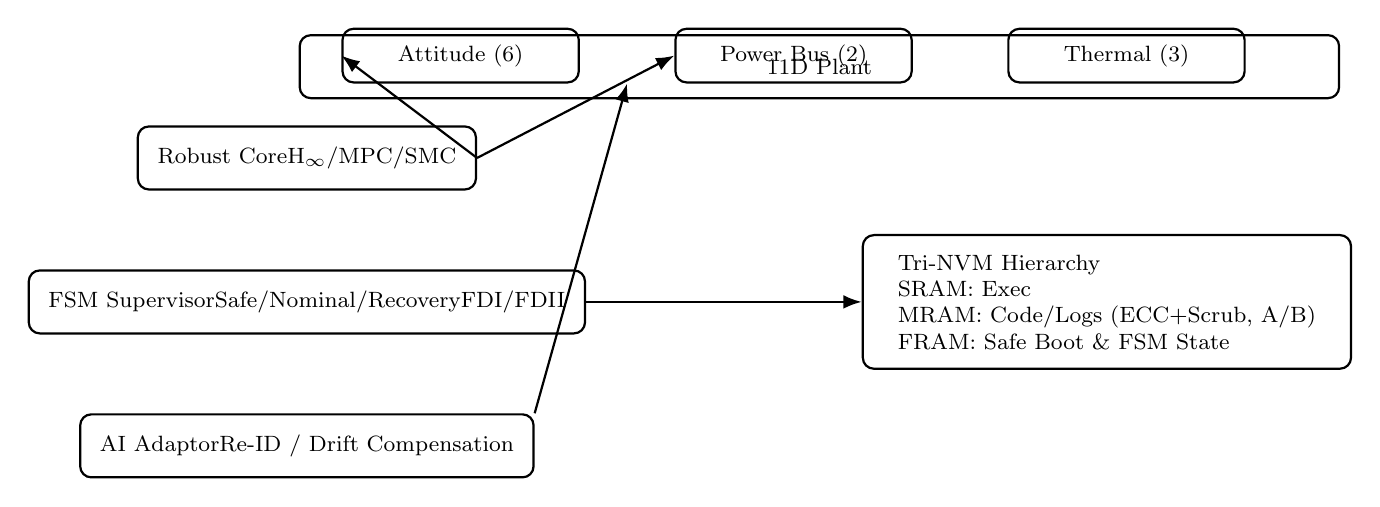
\begin{tikzpicture}[small,thickline]
  % Plant headline
  \node[box, minimum width=13.2cm, minimum height=8mm] (plantbar) {11D Plant};

  % Substates
  \node[box, minimum width=3.0cm, above left=2mm and 1.2cm of plantbar.south east, anchor=south east] (thermal) {Thermal (3)};
  \node[box, minimum width=3.0cm, left=1.2cm of thermal] (bus) {Power Bus (2)};
  \node[box, minimum width=3.0cm, left=1.2cm of bus] (att) {Attitude (6)};

  % Left blocks
  \node[block, below left=13mm and 26mm of att.west, anchor=west] (core) {Robust Core\\\(\mathrm{H_\infty}/\)MPC/SMC};
  \node[block, below=10mm of core] (fsm) {FSM Supervisor\\ Safe/Nominal/Recovery\\FDI/FDII};
  \node[block, below=10mm of fsm] (ai)  {AI Adaptor\\ Re-ID / Drift Compensation};

  % Tri-NVM
  \node[block, right=35mm of fsm, minimum width=6.2cm, align=left] (nvm) {Tri-NVM Hierarchy\\
  SRAM: Exec\\
  MRAM: Code/Logs (ECC+Scrub, A/B)\\
  FRAM: Safe Boot \& FSM State};

  % Connections
  \draw[->] (core.east) -- (att.west);
  \draw[->] (core.east) -- (bus.west);
  \draw[->] (fsm.east) -- (nvm.west);
  \draw[->] (ai.north east) -- ($(att.south)!0.50!(bus.south)$);
\end{tikzpicture}
\caption{AITL on Space architecture with Robust Core, Supervisor FSM, AI Adaptor, and the Tri-NVM hierarchy.}
\label{fig:arch}
\end{figure*}

\section{Introduction}
Long-duration missions require high availability under total ionizing dose (TID), single event effects (SEE), and thermal cycling. Conventional PID+Flash architectures face reliability limits due to charge-trap drift and write endurance. We summarize related work and motivate AITL on Space as a resilient alternative.

\section{System Architecture}
AITL comprises three layers:
\begin{itemize}
  \item Robust Core for H$_\infty$/MPC/SMC control,
  \item FSM Supervisor (Safe/Nominal/Recovery; FDI/FDII),
  \item AI Adaptor for long-term re-identification and drift compensation.
\end{itemize}
A tri-NVM hierarchy is adopted: SRAM for execution, MRAM for code/logs (ECC + scrub, A/B slots), and FRAM for safe boot and FSM state. The target implementation is a 22\,nm FDSOI SoC hardened for radiation and temperature cycling.

\section{Mathematical Model}
We use an 11D discrete-time plant that couples attitude (6), power bus (2), and thermal nodes (3):
\begin{align}
x_{k+1} &= A x_k + B u_k + E w_k, \\
y_k &= C x_k + D u_k + v_k.
\end{align}
The model extends to 20D by adding translational axes and bias states. $w_k$ and $v_k$ represent disturbance and sensor noise, respectively.

% ===== Fig.2 =====
\begin{figure}[!t]
\centering
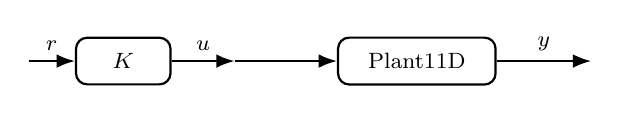
\begin{tikzpicture}[small,thickline]
  \node[box, minimum width=12mm] (K) {\(K\)};
  \node[coordinate, right=8mm of K] (sum) {};
  \node[box, minimum width=20mm, right=13mm of sum] (P) {Plant\\ \footnotesize 11D};
  \draw[->] (-1.2,0) -- (K.west) node[above,midway] {\(r\)};
  \draw[->] (K.east) -- (sum) node[above,midway] {\(u\)};
  \draw[->] (sum) -- (P.west);
  \draw[->] (P.east) -- ++(1.2,0) node[above,pos=0.5] {\(y\)};
\end{tikzpicture}
\caption{Closed-loop schematic used for \(H_\infty\) synthesis on the 11D plant.}
\label{fig:cl}
\end{figure}

\section{H$\infty$ Mixed-Sensitivity Design}
Weights $(W_1,W_2,W_3)$ shape sensitivity, control effort, and complementary sensitivity. EduController exports JSON plant/weights; AITL-H synthesizes an output-feedback $K$ and a fixed-point realization suitable for FPGA/ASIC.

\section{Verification Pipeline}
FPGA HIL injects SEU bursts and sensor outages; metrics include safe-mode time ($<1\,\mathrm{s}$), recovery rate ($\geq 99\%$), and ECC statistics under scrubbing. Physical design proceeds to 22FDX tape-out; SystemDK FEM closes thermal/packaging effects with radiation/temperature scenarios.

% ===== Fig.3 =====
\begin{figure}[!t]
\centering
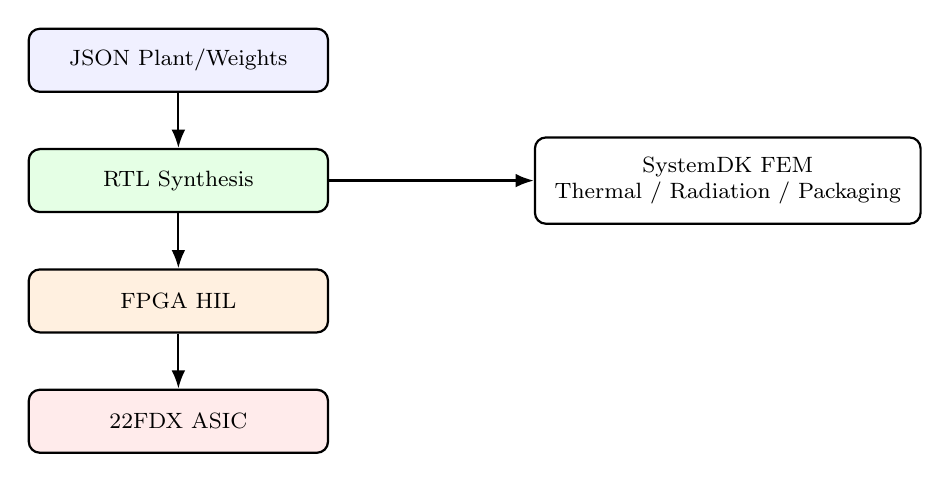
\begin{tikzpicture}[small,thickline,node distance=7mm]
  \node[block, fill=blue!6, minimum width=38mm] (json) {JSON Plant/Weights};
  \node[block, fill=green!10, below=of json, minimum width=38mm] (rtl)  {RTL Synthesis};
  \node[block, fill=orange!12, below=of rtl,  minimum width=38mm] (hil)  {FPGA HIL};
  \node[block, fill=red!8,    below=of hil,  minimum width=38mm] (asic) {22FDX ASIC};

  \node[block, right=26mm of rtl, align=center, minimum width=46mm] (fem)
        {SystemDK FEM\\ Thermal / Radiation / Packaging};

  \draw[->] (rtl.east) -- (fem.west);
  \draw[->] (json) -- (rtl);
  \draw[->] (rtl)  -- (hil);
  \draw[->] (hil)  -- (asic);
\end{tikzpicture}
\caption{Verification pipeline from JSON design to RTL, FPGA HIL, and ASIC; FEM closes the loop with thermal and radiation scenarios.}
\label{fig:flow}
\end{figure}

\section{Conclusion}
AITL on Space provides a practical path to resilient autonomy for deep-space missions by combining robust control, supervisory safety logic, AI-based re-identification, and a tri-NVM memory hierarchy.

\bibliographystyle{IEEEtran}
\bibliography{refs}

% ===== Biography =====
\section*{Author Biography}
\textbf{Shinichi Samizo} received the M.S. degree in Electrical and Electronic
Engineering from Shinshu University, Japan. He worked at Seiko Epson
Corporation as an engineer in semiconductor memory and mixed-signal
device development, and contributed to inkjet MEMS actuators and
PrecisionCore printhead technology. He is currently an independent
semiconductor researcher focusing on process/device education, memory
architecture, and AI system integration. Contact:
\href{mailto:shin3t72@gmail.com}{shin3t72@gmail.com}.
\end{document}
